\section{Module 10. Upsampling}

\textbf{Results}
\newline
To visualize the upsampling functionality several output with different parameters are showed (Fig. \ref{fig: Module10_6}, \ref{fig: Module10_7}).

\begin{figure}[H]
\centering{}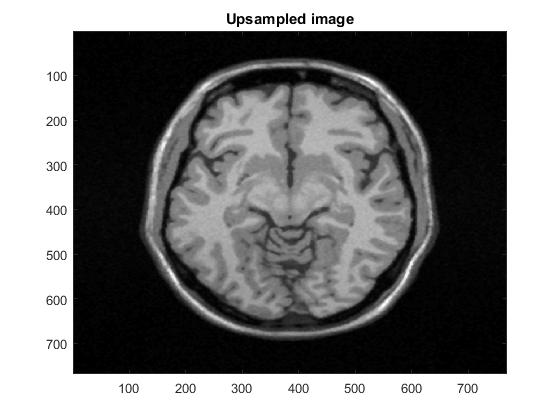
\includegraphics[scale=0.5]{figures/Module_10/Module10_6}\caption{The upsampled image with extensions equal to 3 and window equal to 2}. 
\label{fig: Module10_6}
\end{figure}

\begin{figure}[H]
\centering{}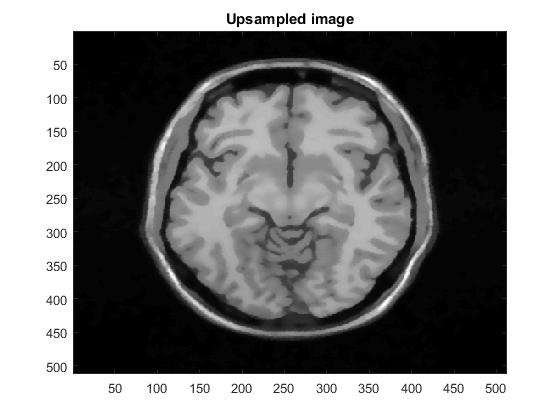
\includegraphics[scale=0.5]{figures/Module_10/Module10_7}\caption{The upsampled image with extensions equal to 2 and window equal to 5}. 
\label{fig: Module10_7}
\end{figure}

To better see the comparison (Fig.\ref{fig: Module10_6_b}, \ref{fig: Module10_7_b})

\begin{figure}[H]
\centering{}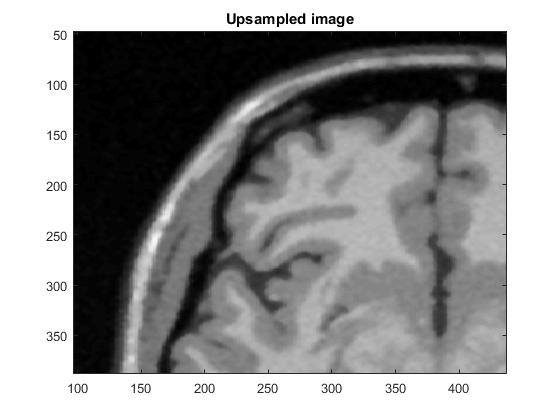
\includegraphics[scale=0.4]{figures/Module_10/Module10_6_b}\caption{The upsampled image with extensions equal to 3 and window equal to 2}. 
\label{fig: Module10_6_b}
\end{figure}

\begin{figure}[H]
\centering{}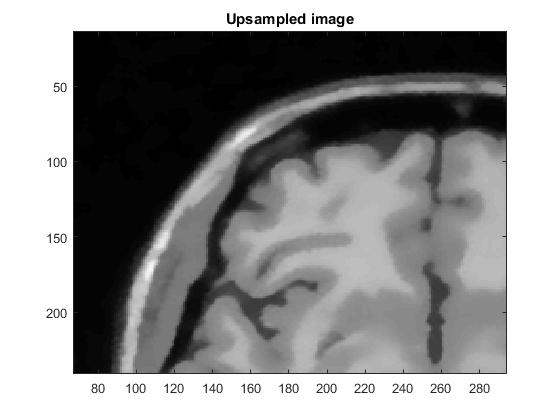
\includegraphics[scale=0.4]{figures/Module_10/Module10_7_b}\caption{The upsampled image with extensions equal to 2 and window equal to 5}. 
\label{fig: Module10_7_b}
\end{figure}

\textbf{Comparison with the other methods}
\newline To confirm the better functionality of the proposed method the results will be compared. The other are Linear, Nearest Neighbour, Cubic and Spline interpolation methods (Fig \ref{fig: Module10_l}, \ref{fig: Module10_NN}, \ref{fig: Module10_c}, \ref{fig: Module10_s}). To better see the comparison (Fig. \ref{fig: Module10_thebest}).

\begin{figure}[H]
\centering{}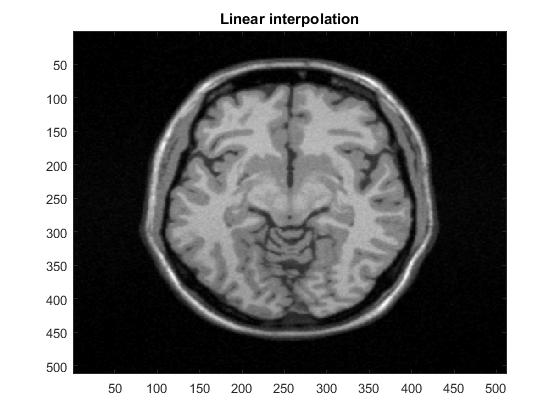
\includegraphics[scale=0.4]{figures/Module_10/Module_10_l}\caption{Linear interpolation}. 
\label{fig: Module10_l}
\end{figure}

\begin{figure}[H]
\centering{}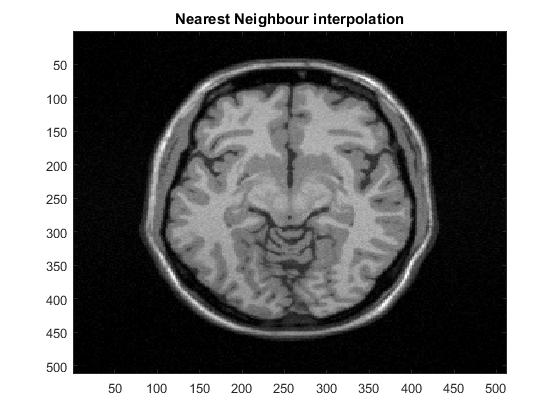
\includegraphics[scale=0.4]{figures/Module_10/Module_10_NN}\caption{Nearest neighbour interpolation}. 
\label{fig: Module10_NN}
\end{figure}

\begin{figure}[H]
\centering{}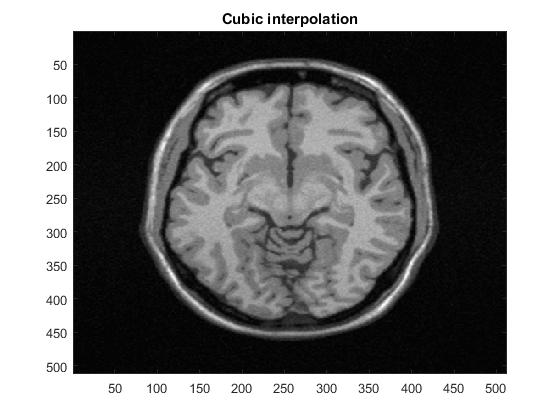
\includegraphics[scale=0.4]{figures/Module_10/Module_10_c}\caption{Cubic interpolation}. 
\label{fig: Module10_c}
\end{figure}

\begin{figure}[H]
\centering{}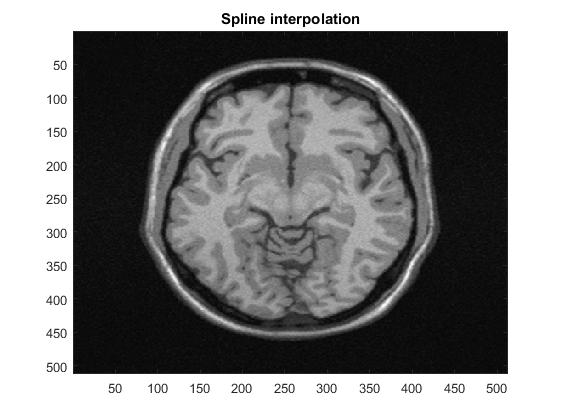
\includegraphics[scale=0.4]{figures/Module_10/Module_10_s}\caption{Spline interpolation}. 
\label{fig: Module10_s}
\end{figure}

\begin{figure}[H]
\centering{}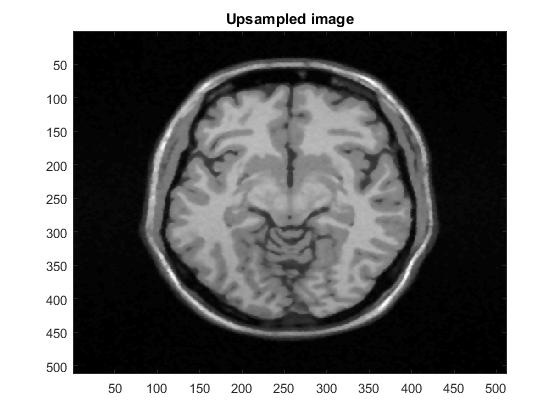
\includegraphics[scale=0.4]{figures/Module_10/Module_10_thebest}\caption{Proposed method}. 
\label{fig: Module10_thebest}
\end{figure}

\textbf{Conclusions}
\newline In conclusion, implementation of a new interpolation method met with success. Unquestionably, the proposed method gives better results than other popular interpolation methods.